\documentclass[12pt,romanian]{report}
\usepackage[utf8]{inputenc}
\usepackage[a4paper,bindingoffset=0.2in,%
            left=0.4in,right=1in,top=1in,bottom=1in,%
            footskip=.25in]{geometry}
\usepackage[romanian]{babel}
\usepackage{amsmath}
\usepackage{amssymb}
\usepackage{float}
\usepackage{graphicx}
\usepackage{subcaption}
\usepackage{hyperref}
\usepackage{listings}
\usepackage{color}
\usepackage{booktabs}
\usepackage{biblatex}

% \usepackage{fancyhdr}

\usepackage[acronym]{glossaries}

\usepackage{helvet}
\renewcommand{\familydefault}{\sfdefault}

% \definecolor{dkgreen}{rgb}{0,0.6,0}
% \definecolor{gray}{rgb}{0.5,0.5,0.5}
% \definecolor{mauve}{rgb}{0.58,0,0.82}

% \lstset{frame=tb,
%   language=Matlab,
%   aboveskip=3mm,
%   belowskip=3mm,
%   showstringspaces=false,
%   columns=flexible,
%   basicstyle={\small\ttfamily},
%   numbers=none,
%   numberstyle=\tiny\color{gray},
%   keywordstyle=\color{blue},
%   commentstyle=\color{dkgreen},
%   stringstyle=\color{mauve},
%   breaklines=true,
%   breakatwhitespace=true,
%   tabsize=3
% }

\addbibresource{references.bib}

\graphicspath{ {./img/} }

% \pagestyle{fancy}

\makeglossaries

\newacronym{ip}{IP}{Internet Protocol}
\newacronym{fp}{FP}{Functional Programming}
\newacronym{frp}{FRP}{Functional Reactive Programming}
\newacronym{cad}{CAD}{Computer Assisted Design}
\newacronym{dto}{DTO}{Data Transfer Object}
\newacronym{oop}{OOP}{Object Oriented Programming}
\newacronym{iot}{IoT}{Internet of Things}
\newacronym{ssl}{SSL}{Secure Sockets Layer}
\newacronym{aws}{AWS}{Amazon Web Services}
\newacronym{api}{API}{Application Programming Interface}
\newacronym{adc}{ADC}{Analog to Digital Convertor}
\newacronym{dac}{DAC}{Digital to Analog Convertor}
\newacronym{gsm}{GSM}{Global System for Mobile Communications}
\newacronym{sim}{SIM}{Subscriber Identity Module}
\newacronym{pcb}{PCB}{Printed Circuit Board}
\newacronym{osi}{OSI}{Open Systems Interconnection}
\newacronym{mvc}{MVC}{Model View Controller}
\newacronym{jwt}{JWT}{JSON Web Token}
\newacronym{napi}{N-API}{Node-API}
\newacronym{dtmf}{DTMF}{Dual-Tone Multi-Frequency}
\newacronym{json}{JSON}{JavaScript Object Notation}
\newacronym{gpio}{GPIO}{General-Purpose Input/Output}
\newacronym{voip}{VoIP}{Voice Over IP}
\newacronym{pots}{POTS}{Plain Old Telephone Service}
\newacronym{rest}{REST}{Representational State Transfer}
\newacronym{rfid}{RFID}{Radio-Frequency Identification}
\newacronym{mosfet}{MOSFET}{Metal Oxide Semiconductor Field Effect Transistor}
\newacronym{arpanet}{ARPANet}{Advanced Research Projects Agency Network}
\newacronym{hmac}{HMAC}{Hash-Based Message Authentication Codes}
\newacronym{sha256}{SHA-256}{Secure Hash Algorithm 256 biti}
\newacronym{hs256}{HS256}{HMAC SHA-256}


% title and other info
\title{PROIECT DE DIPLOMA\\Sistem IoT pentru controlul\\accesului in clădire}
\date{2021\\ Noiembrie}
\author{Alexandru Cristian IONESCU}


\begin{document}

\maketitle

% \chapter*{Abstract}
% Trebuie sa avem asa ceva?

\tableofcontents

\chapter{Introducere}
\section {Obiectivele lucrării de licența}

\subsection {Realizarea unui studiu de piata}

In continuare vom face un scurt studiu de piata pe nisa sistemelor de tip interfon "inteligent".

\subsection {Dezvoltarea unui sistem pentru interfatarea in reteaua IoT}

\section {Descrierea domeniului din care face parte tema de licența}

\href{https://zeusintegrated.com/blog/item/a-brief-history-of-smart-home-automation}{History of smart home automation}

\href{https://www.familyhandyman.com/article/the-history-of-smart-home-technology/}{Apple/Google home}

\href{https://techcrunch.com/2013/05/11/from-the-garage-to-200-employees-in-3-years-how-nest-thermostats-were-born/}{Nest TC}

Studiu de caz: Nest si cum au crescut


Aceasta lucrare face parte dintr-un domeniu mai vechi, dar care a prins amploare recent, domeniul automatizarilor domestice (daca nu e industrial?) si IoT. 

\section {Prezentare pe scurt a capitolelor}



\chapter{Descrierea problemei abordate}
\section {Formularea problemei}

In urma studiului de piata din capitolul anterior am concluzionat ca exista un segment de utilizatori care ar fi interesati in a folosi un astfel de sistem. In cele ce urmeaza voi prezenta 

\section {Studiu asupra realizărilor similare din domeniu}

\section {Stabilirea cerințelor funcționale si nefuncționale ale sistemului}

\subsection{Controlul accesului intr-o cladire}

Scopul principal al acestui sistem este de a oferi sau nu acces intr-o incinta, prin urmare consider aceasta cea mai importanta cerinta functionala.

\subsection{Expunerea unui serviciu REST pentru interfatarea cu alte sisteme}

Expunerea si abstractizarea terminalului \acrshort{pots} este realizata printr-un set de servicii \acrfull{rest} care controleaza starea sa. Acest lucru ne permite interfatarea cu aplicatia mobila, interfata de administrare web si alte servicii precum Google Home/Google Assistant/Apple Home.

\subsection{Implementarea unei functii pentru raspuns automat}

Aceasta functie va permite utilizatorului sa stabileasca o perioada de timp pentru care sistemul va oferi accesul neconditionat.

\subsection{Dezvoltarea unui client mobil Android}

Principalul client care va interactiona cu serviciile \acrshort{rest} va fi aplicatia mobila ce va avea rolul de a notifica userul cand ii suna interfonul si de a controla starea sistemului.

\subsection{Control granular asupra datelor stocate}

Arhitectura aplicatiei necesita interactiunea cu o baza de date, care poate fi tinuta in cloud, pentru convenabilitate sau local.
Folosind tehnologii de containerizare precum Docker, putem stoca baza de date local, informatiile fiind stocate intr-un mediu controlat.

\subsection{Criptarea comunicatiilor cu serviciile web}

Avand in vedere nivelul de acces pe care l-ar oferi un exploit al acestei solutii, comunicatiile intre server si clienti trebuie realizate printr-un canal criptat de tip \acrfull{ssl}. Credentialele userului si ulterior tokenul de acces trebuie trimise doar dupa verificarea autenticitatii serverului si a pachetelor trimise.

\subsection{Oferirea si revocarea accesului la sistem}

Dorim de exemplu sa oferim acces neconditionat unui prieten apropiat pentru a intra in bloc fara a mai suna la interfon. De asemenea ar trebui sa putem realiza si inversul acestei operatii.

\subsection{Expunerea unui flux duplex audio prin tehnologia VoIP}

Pasul final in dezvoltarea acestui sistem ar fi interfatarea cu un \acrfull{adc} si un \acrfull{dac} si expunerea streamurilor de date prin \acrfull{voip}


\chapter{Stadiul actual in domeniu si selectarea soluției tehnice}
\section {Stadiul actual al tehnologiilor utilizate pentru dezvoltarea soluției}


\section {Prezentarea tehnologiilor si platformelor de dezvoltare alese}

\chapter{Considerente legate de implementarea soluției tehnice}
\section {Arhitectura sistemului}

Sistemul prezentat presupune atat o partare hardware, cat si una software. Hardwareul realizeaza adaptarea dintre terminalul analog POTS si placa digitala de dezvoltare Raspberry Pi, iar ca software am folosit NodeJS pentru server si Android pentru a implementa un client al serverului

\subsection {Raspberry Pi HUT}

Pentru a proiecta un \acrfull{pcb} am folosit softwareul Fritzing. Acesta permite proiectarea schemei electrice si ulterior trasarea conexiunilor pe layoutul fizic al placii.

Actionarea butoanelor terminalului \acrshort{pots} se realizeaza cu ajutorul unor opto-cuploare, izoland circuitul interfonului care este proiectat pentru a functiona cu spike-uri de pana la 90V de circuitul Raspberry Pi.

Detectarea unui apel este realizata prin legarea unui \acrfull{mosfet} la bornele difuzorului terminalului \acrshort{pots} si inserierea cu un amplificator operational in regim de comparator cu referinta de 0.1V. Am folosit de asemenea si un Filtru Trece Jos deoarece terminalul este sensibil la zgomote, declansand accidental notificarea.

\subsubsection {Optocuploare homemade}

Datorita crizei globale de semiconductori, o placuta breakout care care include doua optocuploare costa aproximativ 50 RON. Considerand simplitatea functionarii acestui circuit, am decis sa construiesc propria solutie, folosind componetele de baza: un rezistor pentru limitat curentul, un LED si un fotorezistor. Platforma Raspberry Pi furnizeaza pinilor sai \acrshort{gpio} 3.3V si un curent maxim de 16mA, iar un LED rosu are o cadere de tensiune de 2.4V:

\begin{center}
\begin{gather*}
I_{GPIO} =10\ mA=10^{-2} A\\
V_{R} =V_{GPIO} -V_{LED} =3.3V-2.4V=0.9V\\
I_{GPIO} =\frac{V_{R}}{R} \ sau\ R=\frac{V_{R}}{I_{GPIO}} =\frac{0.9V}{10^{-2}A} =90\Omega
\end{gather*}
\end{center}

Am lipit rezistorul de 90$\Omega$ la anodul ledului si am incastrat LED-ul impreuna cu fotorezistorul intr-o incinta fara lumina.

\begin{figure}[h!]
\centering
\begin{subfigure}{.5\textwidth}
  \centering
  \includegraphics[width=.8\linewidth]{04/01_optocoupler_scheme.jpg}
  \caption{Schema optocuplor \cite{OptocouplerCircuitsToday}}
  \label{fig:sub1}
\end{subfigure}%
\begin{subfigure}{.5\textwidth}
  \centering
  \includegraphics[width=.8\linewidth]{04/02_optocoupler_assembly.png}
  \caption{Ansanblu realizat manual}
  \label{fig:sub2}
\end{subfigure}
\caption{Schema electrica optocuplor (a) si rezultat ansablu (b)}
\label{fig:test}
\end{figure}

Deoarece aveam nevoie sa scurtcircuitez un contactor pe partea terminalului \acrshort{pots} am omis rezistenta legata fotorezistorului. Atunci cand ledul este aprins, rezistenta fotorezistorului scade, comportandu-se aproape ca un conductor ideal, atingand lamelele contactorului corespunzator receptorului.

\subsection {Webserver NodeJS}

NodeJS este un

\subsubsection {NestJS}

Metadate si chestii, dependency injection si MVC la aplicatie

\subsubsection {Mutex}

Din natura asincrona a limbajului si posibilitatea sistemului de a avea mai mult de un utilizator, trebuie luat in considerare cazul in care mai multi utilizatori incearca sa interactioneze cu sistemul in acelasi timp. Asadar, trebuie implementat un mecanism similar semaforului binar, numit mutex. Diferenta dintre acestea fiind ca in cazul mutexului, doar detinatorul original poate sa il elibereze spre a fi folosit.

Acest comportament este de dorit pentru a informa clientii serviciului in cazul in care requestul nu poate fi satisfacut deoarece resursa este ocupata de altcineva.

\begin{figure}[h!]
  \centering
  \fbox {
    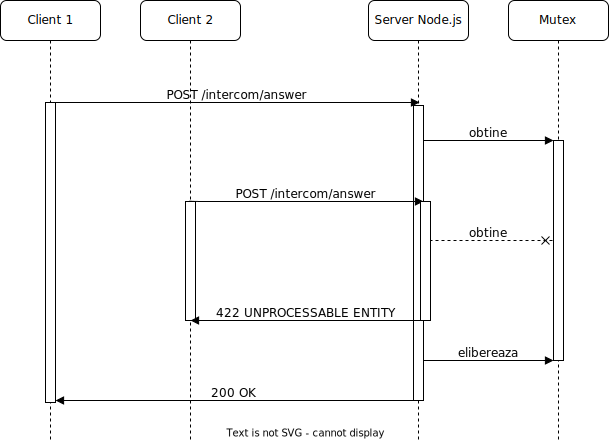
\includegraphics[width=0.6\textwidth]{04/03_mutex_diagram.pdf}  
  }
  \caption{Ilustrare resursa disputata intre doi utilizatori}
\end{figure}


\subsubsection {Validare}

Foloseste functii din Typescript si NestJS pentru a adauga si citi metadate prin intermediul decoratorilor de metode.

\subsubsection {Autentificare}

La fel ca mai sus

\subsubsection {Roluri}

Din nou decorator


\subsection {Android}

Android este o platforma mobile care s-a maturizat pe parcusul a 12 versiuni majore si principalul competitor de piata al iOS.


\section {Implementarea sistemului}


\section {Testarea sistemului}

\chapter{Studiu de caz}
\section{Oferirea accesului unui utilizator}

Operatia de oferire a accesului unui nou utilizator presupune folosirea interfetei de administrare. Dupa setarea numeului noului utilizator si a parolei, noul cont este gata pentru folosit, iar pentru convenabilitate codul QR geenrat poate fi scanat cu aplicatia pentru a se autentifica automat

\begin{figure}[H]
\begin{center}
  \subfloat[Introducerea credentialelor noi]{\label{fig:useradda}\includegraphics[width=\doublefigure]{05/06_admin_add_user.png}}
  \hfil
  \subfloat[Confirmarea adaugarii noului cont]{\label{fig:useraddb}\includegraphics[width=\doublefigure]{05/07_admin_add_user_success.png}}
  \caption{Creare utilizator nou}
  \label{fig:useradd}
\end{center}
\end{figure}

Dupa descarcarea aplicatiei din Google Play Store, se va putea realiza autentificarea. Un alt avantaj al unui astfel de sistem este eliminarea nevoii cartelelor fizice, usor pierdut sau incurcat.

\begin{figure}[H]
\begin{center}
  \subfloat[Ecran autentificare aplicatie]{\label{fig:androidqra}\includegraphics[width=\doublefigure]{05/08_android_log_in.png}}
  \hfil
  \subfloat[Scanarea codului QR]{\label{fig:androidqrb}\includegraphics[width=\doublefigure]{05/09_android_qr.png}}
  \caption{Autentificare prin scanare cod QR}
  \label{fig:androidqr}
\end{center}
\end{figure}

\section{Raspuns automat}

Majoritatea vizitelor si apelurilor la interfon sunt previzibile, de exemplu venirea curierului sau a unui postas este anuntata printr-un interval aproximativ de timp. Deoarece utilizatorul duce o viata ocupata si stie ca urmeaza sa fie sunat, poate programa sistemul sa raspunda si sa deschida automat usa la urmatorul apel pentru o durata predefinita.

\begin{figure}[H]
\begin{center}
  \subfloat[Apasarea butonului albastru auto-answer va arata meniul pentru configurarea functionalitatii]{\label{fig:autoanswera}\includegraphics[width=\doublefigure]{05/01_android_autoanswer.png}}
  \hfil
  \subfloat[Alegerea unui interval pentru care functia va fi activa]{\label{fig:autoanswerb}\includegraphics[width=\doublefigure]{05/02_android_auto_set.png}}
  \caption{Pasi pentru setare functie auto-answer}
  \label{fig:autoanswer}
\end{center}
\end{figure}

Se confirma activarea functiei prin colorarea butonului auto-answer in portocaliu. Intr-o maniera similiara, daca se doreste oprirea inainte de termen, se poate face acest lucru din meniul anterior.

\section{Raspuns de la distanta}

Prin conectarea la reteaua \acrshort{iot} sistemul este expus Internetului, acesta fiind avantajul solutiei, dar si unul din factori limitanti ai sai. Posibilitatea de deschidere de oriunde clientul are un dispzitiv conectat la Internet inseamna ca in lipsa cartelei standard \acrfull{rfid} se poate apela propriul apartament. Se va folosi aplicatia mobila pentru a se raspunde la propriul apel.

\begin{figure}[H]
\begin{center}
  \subfloat[In cazul in care aplicatia este pornita, utilizatorul este redirectat in IncomingActivity]{\label{fig:ringinga}\includegraphics[width=\doublefigure]{05/04_android_app_ringing.png}}
  \hfil
  \subfloat[In cazul in care aplicatia nu este in foreground, se trimite o notificare de sistem cu doua actiuni]{\label{fig:ringingb}\includegraphics[width=\doublefigure]{05/05_android_notification_ringing.png}}
  \caption{Ecran apel}
  \label{fig:ringing}
\end{center}
\end{figure}

O alta varianta pentru mitigarea acestei probleme a fost folosirea unui tag \acrfull{nfc} care contine codat url-ul de acces impreuna cu un token care nu expira. Astfel prin scanarea lui cu un telefon ce dispune de anena \acrshort{nfc} se va realiza request-ul din browserul default al utilizatorului, rezultand in deschiderea interfonului.

\chapter{Concluzii}
\section{Concluzii 'si contribu'tii}

Având în vedere informa'tiile expuse în capitolele 1, 2, 3 'si cuno'stin'tele dobândite în realizarea arhitecturii unui sistem de tip încuietoare inteligentă, dar 'si rezultatele studiului de caz demonstrează că se pot crea solu'tii folosind tehnologii open-source. Prin alegeri sensibile din punct de vedere tehnic în ceea ce prive'ste securitatea sistemului, utilizatorul normal poate folosi aplica'tia pentru a î'si controla interfonul într-un mod sigur. De asemenea, includerea tehnologiilor open-source înseamnă că utilizatorii avansa'ti au multiple alegeri în ceea ce prive'ste implementarea solu'tiei (pot alege unde sunt stocate datele 'si cine are acces la ele, pot configura din firewall accesul la \acrshort{api} 'si la interfa'ta administrativă).

Prin urmare, această lucrare arată că se poate concepe o solu'tie \acrshort{iot} la nivelul standardelor secolului 21, atât din punct de vedere al securită'tii cât 'și al proprietă'tii datelor stocate. Integrarea să u'soară poate doar să beneficieze adoptării mai rapide a acestui sistem.

Sinteza informa'tiilor conform literaturii de specialitate cât și analiza solu'tiilor existente din în ceea ce prive'ste ni'să încuietorilor inteligente a produs un exercițiu interesant în explorarea posibilității realizării unui sistem compatibil \acrshort{iot} care să ofere majoritatea functionalitatilor disponibile pe piață, păstrând în același timp spiritul hobist original.

S-a demonstrat că se pot folosi componente electronice simple pentru a realiza un optocuplor mai ieftin, dar care oferă accea'și func'tionalitate în cazul acestei aplica'tii. Prin ținerea costurilor finale, se oferă o propunere mai atractivă utilizatorilor doritori să încerce acest sistem.

Conceperea arhitecturii unui sistem complex care să satisfacă cerin'tele func'tionale prezentate de nișa dispozitivelor Smart Home din ziele noastre, culminata cu implementarea fizică a acestui concept 'si testarea în via'tă de zi cu zi demonstrează viabilitatea teoretică.

Prin testarea riguroasă a componentelor individuale ale sistemului, cât și testarea sa ca un întreg, se asigură un standard înalt de calitate pentru o aplicație cu o responsabilitate critică în viață utilizatorului final. Construind o fundație riguroasă pentru o platformă de tip Smart Lock care să ofere posibilitatea dezvoltărilor ulterioare, aducând valoare adăugată adepților timpurii.

\section{Dezvoltări ulterioare}

Dezvoltări ulterioare ale sistemului ar presupune construirea unui terminal \acrshort{pots} întreg ca \acrshort{hat} pentru RaspberryPi. Astfel vom putea atinge 'si cerin'ta de a oferi utilizatorului fluxuri audio pentru a comunica cu persoana de la celălalt capăt al interfonului. 

% \chapter{Bill of Materials}
% \input{tex/09_bill_of_materials}

\clearpage

\printglossary[type=\acronymtype,title={Acronime}]
\printglossary

\printbibliography[heading=bibnumbered]

\end{document}